\subsection{Polarization Vectors and Transverse Asymmetries}

The BBCs enable local polarimetry at STAR.  Vertical polarization in the beam generates an asymmetry in the counts recorded by the left and right halves of the BBC on which it impinges, while radial polarization generates an asymmetry in the top and bottom halves of the detector.  An accurate accounting of residual non-longitudinal polarization in the beams is important, because a double transverse spin asymmetry \(A_{\Sigma}\) could generate a false \(A_{LL}\).  The size of this false signal is given by the equation
%
\begin{equation}
  \delta A_{LL}^{\mathrm{non-longitudinal}} = | \tan(\theta_B) \tan(\theta_Y) \cos(\phi_B - \phi_Y) A_{\Sigma} |.
  \label{eqn:pol-vector-uncertainty}
\end{equation}
%
The beam polarization angles at STAR are determined through an analysis of cross ratios in the BBCs \cite{Kiryluk:2005gg}.  These ratios are directly sensitive to the azimuthal angle of the beam, and a comparison of the ratios in longitudinal and transverse running allows an extraction of the angle of inclination when the spin rotators are active.  The measured ratio is 
%
\begin{equation}
  \epsilon_{BBC} = \frac{r_{ij} -1}{r_{ij} + 1} \simeq \left\{
  \begin{array}{l l}
    A_N^{BBC} \times P_v \times \langle \cos \phi \rangle & i,j = \mbox{Left, Right} \\
    A_N^{BBC} \times P_r \times \langle \sin \phi \rangle & i,j = \mbox{Up, Down} \\
  \end{array} \right.
\end{equation}
%
in which \(r_{ij} = \sqrt{\frac{N_i^{\uparrow} N_j^{\downarrow}}{N_i^{\downarrow} N_j^{\uparrow}}}\) and \(N_{i(j)}^{\uparrow(\downarrow)}\) are the spin dependent yields on the Left (Right) or Up (Down) side of the detector. \(P_{v(r)}\) is the vertical (radial) beam polarization.  The effective analyzing power of the BBCs is approximately 0.7\%, as shown in Figure~\ref{fig:bbc-analyzing-power} for the 2006 RHIC run. Table~\ref{tab:pol-vectors} tabulates the extracted polarization vectors from measurements of the BBC cross-ratios.  There are two separate extractions for the 2006 data because the spin rotator magnets were adjusted midway through the run.  The data show a steady improvement in the performance of the spin rotators.

\begin{figure}
  \centering
  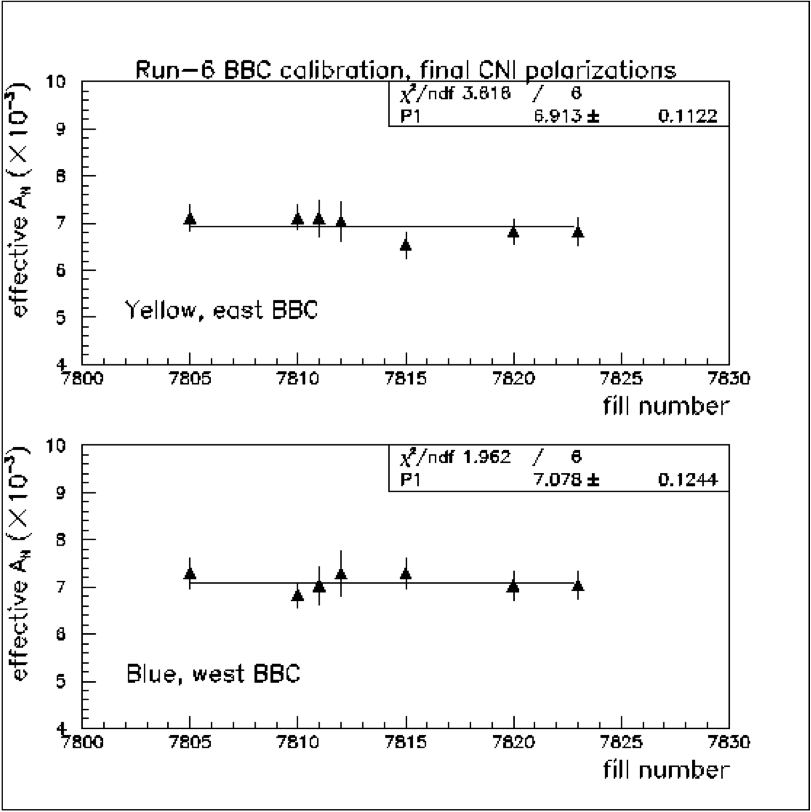
\includegraphics[width=0.6\textwidth]{figures/bbc-analyzing-power}
  \caption{Effective analyzing power of the BBC local polarimeters in the 2006 RHIC run.  The analyzing power is approximately constant from year to year.}
  \label{fig:bbc-analyzing-power}
\end{figure}

% Table of Beam Polarization Vectors
\begin{table}
  \begin{center}
    \begin{tabular}{|l|c|c|r|}
      \hline
      Run Period & Blue ($\theta, \phi$) & Yellow ($\theta, \phi$) &
      $\frac{\delta A_{LL}}{A_{\Sigma}}$\\
      \hline
      2005 & (7.9, 74.0) & (17.2, 138.7) & 0.0184 \\
      2006a (7132001-7138034) & (6.9, 87.7) & (10.0, 34.4) & 0.0128 \\
      2006b (7138035-7156040) & (0.9, 69.3) & (3.9, -47.8) & 0.0005 \\
      \hline
    \end{tabular}
  \end{center}
  \caption{Beam polarization vectors as determined from an analysis of up-down and left-right asymmetries in the BBCs.  The spin rotators were adjusted midway through the second longitudinal running period in 2006.  A weighted average of the two 2006 results yields $\delta A_{LL} / A_{\Sigma} = 0.006$.}
  \label{tab:pol-vectors}
\end{table}

Double transverse asymmetries are plotted in Figure~\ref{fig:asigma}.  The transverse dataset in the 2005 RHIC run is very limited; only 27 runs pass all quality checks.  As a result, the measurement of \(A_{\Sigma}\) has large statistical uncertainties.  Some analyses at STAR have used the 2006 transverse data to constrain \(A_{\Sigma}\) when assigning systematic uncertainties for measurements based on 2005 data, but the very different jet patch trigger thresholds for the two years make a cross-comparison of inclusive charged pion data difficult.

Tables~\ref{tab:syst-pol-2005} and \ref{tab:syst-pol-2006} contain the final systematic uncertainties accounting for a possible bias in \(A_{LL}\) arising from transverse asymmetries in the beam.  The systematic is calculated by taking the larger of the central value for \(A_{\Sigma}\) in a bin, and its uncertainty in that bin, and multiplying by the polarization vector scaling factor in Table~\ref{tab:pol-vectors}.  In the case of the 2006 RHIC run, a weighted average of the two scaling factors is used.  It turns out that non-longitudinal beam components do not contribute significantly to the total systematic uncertainty in the 2006 analysis, but in 2005 the combination of larger non-longitudinal beam components and a statistically-limited transverse dataset lead to a very conservative uncertainty envelope.

% due to the large non-statistical variations, ∼1.5 degrees, in the estimate of the polar angle coming from the the up/down asymmetries in the transverse running, we decided to use a conservative estimate of cos(φY − φB) = 1.

% that doesn't make much sense ... UD transverse asymmetries don't contribute to the determination of the polar angle to first order.

% also, the formulae to get the beam angles from these asymmetries are inconsistent.  But Murad's numbers for tan(theta) and phi do yield his numbers for the multiplicative factor in front of Asigma

\begin{figure}
  \subfloat[][Run 5]{
    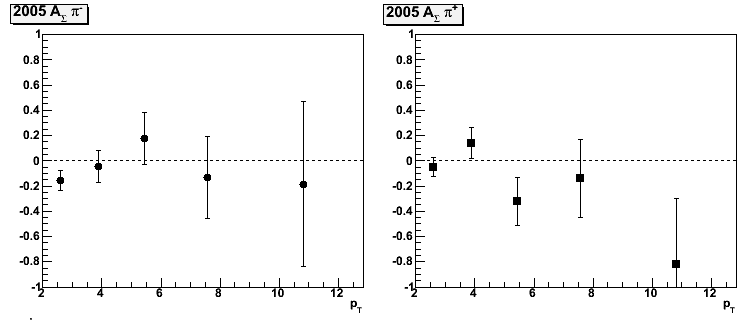
\includegraphics[width=1.0\textwidth]{figures/asigma_2005}
  } \\
  \subfloat[][Run 6]{
    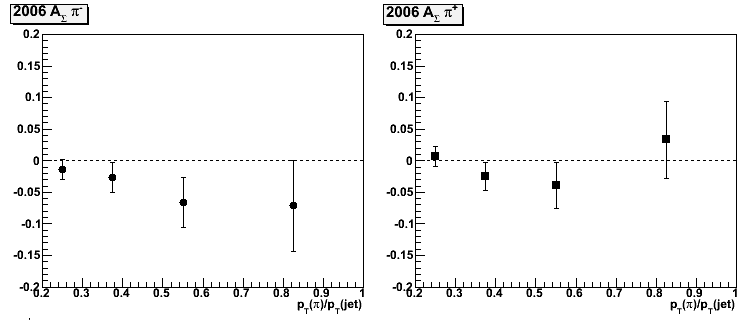
\includegraphics[width=1.0\textwidth]{figures/asigma_2006}
  }
  \caption{Double transverse asymmetries calculating from the transverse running periods of the 2005 (top) and 2006 (bottom) RHIC runs. Note the difference in scale on the vertical axis.}
  \label{fig:asigma}
\end{figure}

\begin{table}
  \centering
  \begin{tabular}{|c||c|c||c|c|}
    \hline
    \multirow{2}{*}{$p_T$} & \multicolumn{2}{c||}{$\pi^{-}$} & \multicolumn{2}{c|}{$\pi^{+}$} \\
    \cline{2-5}
    & $A_{\Sigma}$ & $\delta A_{LL}$ ($10^{-4}$) & $A_{\Sigma}$ & $\delta A_{LL}$ ($10^{-4}$) \\
    \hline
    2.00 - 3.18  & -0.158 $\pm$ 0.077 & 29.1  & -0.050 $\pm$ 0.073 & 13.4  \\
    3.18 - 4.56  & -0.044 $\pm$ 0.125 & 23.0  & ~0.139 $\pm$ 0.124 & 25.6  \\
    4.56 - 6.32  & ~0.176 $\pm$ 0.203 & 37.4  & -0.324 $\pm$ 0.192 & 59.6  \\
    6.32 - 8.80  & -0.134 $\pm$ 0.325 & 59.8  & -0.139 $\pm$ 0.311 & 57.2  \\
    8.80 - 12.84 & -0.185 $\pm$ 0.656 & 120.7 & -0.821 $\pm$ 0.524 & 151.1 \\
    \hline
  \end{tabular}
  \caption{Systematic uncertainty on $A_{LL}$ due to residual transverse beam polarization in the 2005 RHIC run.}
  \label{tab:syst-pol-2005}
\end{table}

\begin{table}
  \centering
  \begin{tabular}{|c||c|c||c|c|}
    \hline
    \multirow{2}{*}{$z$} & \multicolumn{2}{c||}{$\pi^{-}$} & \multicolumn{2}{c|}{$\pi^{+}$} \\
    \cline{2-5}
    & $A_{\Sigma}$ & $\delta A_{LL}$ ($10^{-4}$) & $A_{\Sigma}$ & $\delta A_{LL}$ ($10^{-4}$) \\
    \hline
    0.20 - 0.30 & -0.014 $\pm$ 0.016 & 1.0 & ~0.007 $\pm$ 0.015 & 0.9 \\
    0.30 - 0.45 & -0.027 $\pm$ 0.023 & 1.6 & -0.025 $\pm$ 0.022 & 1.5 \\
    0.45 - 0.65 & -0.066 $\pm$ 0.040 & 4.0 & -0.039 $\pm$ 0.037 & 2.3 \\
    0.65 - 1.00 & -0.072 $\pm$ 0.073 & 4.4 & ~0.033 $\pm$ 0.061 & 3.7 \\
    \hline
  \end{tabular}
  \caption{Systematic uncertainty on $A_{LL}$ due to residual transverse beam polarization in the 2006 RHIC run.  The uncertainties are obtained using the weighted average scaling factor discussed in Table~\ref{tab:pol-vectors}}
  \label{tab:syst-pol-2006}
\end{table}

